\ifdefined\COMPLETE
\else
\documentclass[12pt]{article}

\usepackage{algorithm}
\usepackage{mathtools,amsmath,amssymb,amstext,amsthm,tikz,thmtools}
\usepackage[inline]{enumitem}

\usepackage[utf8]{inputenc} % allow utf-8 input
\usepackage[T1]{fontenc}    % use 8-bit T1 fonts
\usepackage{hyperref}       % hyperlinks
\usepackage{url}            % simple URL typesetting
\usepackage{booktabs}       % professional-quality tables
\usepackage{amsfonts}       % blackboard math symbols
\usepackage{nicefrac}       % compact symbols for 1/2, etc.
\usepackage{microtype}      % microtypography

\newcommand{\mc}{\mathcal}
\newcommand{\mb}{\mathbf}
\newcommand{\tr}{\text{Tr}}
\newcommand{\diag}{\text{diag}}
\newcommand\numberthis{\addtocounter{equation}{1}\tag{\theequation}}

\DeclareMathOperator*{\argmin}{arg\,min}
\DeclareMathOperator*{\argmax}{arg\,max}

\newtheorem{theorem}{Theorem}
\newtheorem{lemma}[theorem]{Lemma}
\newtheorem{definition}[theorem]{Definition}
\newtheorem{proposition}[theorem]{Proposition}
\newtheorem{corollary}[theorem]{Corollary}

\begin{document}
\fi

\section{Hardness of regularised $k$-means}
\label{a-section:hardness}
\begin{theorem}
\label{a-theorem:hardFork1Fixed}
Given a clustering instance $\mc X \subset \mb R^{d}$, define $m(\mc X) := \min_{x \neq y \in \mc X} \|x-y\|_{2}^2$ and $n := |\mc X|$. Finding the optimal solution to the regularised $1$-means objective is NP-Hard for $\frac{m(\mc X)}{2} < \lambda < \frac{m(\mc X)}{2} + \frac{1}{2n^2(n-1)}$. 

In particular, the optimization problem is NP-Hard for $\lambda = \lambda_0(\mc X) := \frac{m(\mc X)}{2} + \frac{1}{4n^3}$.
\end{theorem}

\begin{proof}
The proof uses reduction from the clique problem. Given a graph $G = (V, E)$ and an integer $q$, the clique problem asks the following: does there exist a clique in $G$ of size at least $q$?

Given an instance of the clique problem, we construct an instance of regularised $1$-means as follows. For every $v \in V$, construct $x_v \in \mc X$. Define the metric as 
\[
d^2(x_i, x_j) = 
\begin{cases}
1 \hspace{0.51in}\text{if }(i, j) \in E\\
1 + \Delta \hspace{0.221in}\text{if }(i, j) \not\in E\numberthis\label{a-eqn:dmetric}
\end{cases}
\]
where $0 < n\Delta < 1 $. Now, we will show that $G$ has a clique of size $ \ge q$ $\iff$$\mc X$ has a clustering of cost $\le c = \frac{q-1}{4} + \lambda (n - q)$.

$\Longrightarrow$ Assume $G$ has a clique of size at least $q$. Assign all points in the clique to $C_1$ and the remaining points to $C_2$. This clustering has cost as desired.

$\Longleftarrow$ Let $|C_1| = n'$. Now, there are three possibilities.

Case 1: $n' > q$. If all the distances in $C_1$ are 1, then the cost of the clustering is $\frac{n'-1}{4} + \lambda (n - n') \le c$ as $\lambda > \frac{1}{2}$. Thus, the vertices corresponding to the points in $C_1$ form a clique of size $n' > q$. If at least one distance is $1 + \Delta$ then the cost of the clustering is 
\begin{flalign*}
\frac{n'-1}{4} + \lambda (n - n') + \frac{\Delta}{n'} \le c \implies \lambda \ge \frac{1}{2} + \frac{\Delta}{n'(n'-q)}
\end{flalign*}
This is a contradiction because of the choice of $\lambda$.

Case 2: $n' < q$. If all the distances in $C_1 = 1$, then the cost of the clustering is $\frac{n'-1}{2} + \lambda (n - n') > c$. If atleast one distance is $1 + \Delta$ then the cost of the clustering is even greater as $\lambda > \frac{1}{2}$. 

Case 3: $n' = q$. If atleast one distance is $1 + \Delta$ then the cost of the clustering is $\frac{q-1}{2} + \lambda (n - q) + \frac{\Delta}{m} > c$ . 
Hence, the only possibility remains that $|C_1| = q$ and all the distances in $C_1 = 1$. Hence, $G$ has a clique of size $q$.
\end{proof}

\begin{lemma}
Let $d$ be as in Eqn. \ref{a-eqn:dmetric}. Then $d$ can be embedded into $\mb R^{|\mc X|}$.
\end{lemma}
\begin{proof}
The proof of embedding is very similar to Thm. 8 in \cite{dasgupta2008hardness}. Using Cor. 7 in \cite{dasgupta2008hardness}, we know that $D$ can be embedded into $\mb R^{|\mc X|}$ if and only if $u^TDu \le 0$ for all $u^T1 = 0$.
\begin{align*}
u^TDu &= \sum_{ij} u_{i}d_{ij}u_{j} = \sum_{ij}u_iu_j \Big(1 - \mb 1(i=j) + \Delta \mb 1(i \not\sim_{E} j) \big)\\
&\le \Big(\sum_{i}u_i \Big)^2 - \sum_i u_i^2 +\Delta\sum_{ij}|u_i||u_j| \le -\|u\|^2 + |\mc X|\Delta \|u\|^2 = -(1-|\mc X|\Delta)\|u\|^2,
\end{align*}
which completes our proof.
\end{proof}

We now use Thm. \ref{a-theorem:hardFork1Fixed} to show that regularised $1$-means is Np-Hard for any $\lambda > m(\mc X) / 2$.

\begin{restatable}{theorem}{hardForkone}
\label{a-theorem:hardFork1}
Given a clustering instance $\mc X \subset \mb R^d$. Finding the optimal solution to the regularised $1$-means objective is NP-Hard for all $\lambda > m(\mc X) / 2$.
\end{restatable}
\begin{proof}
Denote $d(x,y)$ to be the $l_2$ distance. Thm. \ref{a-theorem:hardFork1Fixed} showed that optimizing the problem  
\begin{align*}
\min_{C\subseteq \mc X} \enspace \sum_{x \in C}d^2(x, c) + \lambda_0(\mc X) \enspace |\mc X\setminus \mc C| \hspace{0.5in}\text{(FRM)}
\end{align*}
is NP-Hard when $\lambda_0(\mc X) := \frac{m(\mc X)}{2} +\frac{1}{4n^3}$. Given $\lambda>0$, we want to show that for all $\lambda > m(\mc X) / 2$, the following is also NP-Hard to optimize: 
\begin{align*}
\min_{C\subseteq \mc X} \enspace \sum_{x \in C}d^2(x, c) + \lambda \enspace |\mc X\setminus \mc C| \hspace{0.5in}\text{(GRM)}
\end{align*}

Let $\lambda' = \sqrt{n^3(4\lambda - 2m(\mc X))} > 0$, and define a new Euclidean distance $d'(x, y) = \frac{d(x,y)}{\lambda'}$. Then
\begin{flalign*}
\sum_{x \in C}d^2(x, c) + \lambda \enspace |\mc X\setminus \mc C| &= \lambda'^2\Bigg(\sum_C d'^2(x, c) + \frac{|\mc X \setminus \mc C|}{\lambda'^2} \Big(\frac{m(\mc X)}{2} +\frac{\lambda'^2}{4n^3}\Big)\Bigg)\\
&= \lambda'^2\Big(\sum_C d'^2(x, c) + |\mc X \setminus \mc C| \lambda_0(\mc X')\Big).&
\end{flalign*}
Hence, we see that GRM is equivalent to FRM which is NP-Hard.
\end{proof}

\section{The regularised $k$-means algorithm}
\label{a-section:heuristic}
 
\subsubsection{Equivalence of regularised $k$-means with $0,1$-SDP}
\label{a-subsection:modifiedkmeans01sdp}
We follow a similar technique to that of \cite{peng2007approximating} to translate equation \ref{eqn:modifiedkmeans} into a 0-1 SDP. We are given a set $\mc X$ with $n$ data points. The goal is to partition the set into $k$ clusters with the option of throwing some points into the garbage $k+1$ cluster. Let $S$ be an assignment matrix of size $n\times k$ and $y$ be an $n \times 1$ column vector that assigns points to the ``garbage'' cluster.  

 \[s_{ij} = 
    \begin{dcases}
		\hspace{0.1in} 1 \enspace \text{iff }x_i \in C_j, j \leq k\\
		\hspace{0.1in} 0 \enspace \text{otherwise}
	\end{dcases}
 \quad y_{i} = 
    \begin{dcases}
		\hspace{0.1in} 1 \enspace \text{iff }x_i \in C_{k+1}\\
		\hspace{0.1in} 0 \enspace \text{otherwise}
	\end{dcases}
\]

Provided that $C_i\ne\emptyset$, we have the following equality by expanding the mean $c_i = \frac{1}{|C_i|} \sum_{x\in C_i} x$:
\begin{align}
\label{a-eqn:kmeansobj1}
\sum_{x \in C_i} \|x-c_i\|^2 
&= \frac{1}{2|C_i|}\sum_{x, y \in C_i} \|x-y\|^2 
\end{align}

\noindent $c_j = \frac{\sum_{i} s_{ij} x_i}{\sum_{i} s_{ij}}$ is the average of points in the $j^{\text{th}}$ cluster. Hence,
\begin{align*}
	&\sum_j \sum_i s_{ij}(\langle c_j, c_j\rangle -2\langle x_i, c_j\rangle) = 	 \sum_j \langle\sum_i s_{ij} c_j, \enspace c_j\rangle - 2 \sum_j \langle\sum_i s_{ij} x_i, \enspace c_j\rangle \\
	&=\sum_j \langle c_j, \sum_i s_{ij}x_i\rangle - 2 \sum_j \langle\sum_i s_{ij} x_i, \enspace c_j\rangle = -\sum_j \langle\frac{\sum_i s_{ij} x_i}{\sum_i s_{ij}}, \sum_i s_{ij}x_i\rangle = -\sum_j \frac{\| \sum_i s_{ij} x_i\|^2}{\sum_i s_{ij}} \numberthis \label{a-eqn:kmeansobj2}
\end{align*}

\noindent Combining equations \ref{a-eqn:kmeansobj1} and \ref{a-eqn:kmeansobj2}, we get that 
\begin{align*}
  &\sum_{j=1}^k \sum_{x \in C_i} \|x-c_i\|^2 = \sum_{i=1}^n \|x_i\|^2 (1-y_i) - \sum_{j=1}^k \frac{\| \sum_i s_{ij} x_i\|^2}{\sum_i s_{ij}} = \sum_{i=1}^n \|x_i\|^2 (1-y_i) - \sum_{i=1}^n\sum_{j=1}^n \langle x_i, x_j\rangle Z_{ij} \label{a-eqn:halfcost}\numberthis
\end{align*}

where $Z = S (S^T S)^{-1} S^T$. Observe that if $x_i \not\in C_{k+1}$ then $Z_{ij} = \frac{1}{|S_{c(i)}|} \langle s_i, s_j\rangle$ where $S_{c(i)}$ denotes the size of the $i^{th}$ cluster. If $x_i \in C_{k+1}$ then $Z_{ij}=0$. Thus, 
\[
	Z_{ij} = 
	\begin{dcases}
	\frac{1}{|S_{c(i)}|} \langle s_i, s_j\rangle \quad &\text{if }y_i = 0\\
	0 \quad &\text{otherwise }
	\end{dcases}
\]
Observe that $Z_{ij} = Z_{ji}$ and
\begin{align*}
\tr(Z) &= \sum_i Z_{ii} = \sum_{x \not\in C_{k+1}} \frac{1}{|S_{c(i)}|} = k. 
\end{align*}
Also, we have that  and $\langle Z_i, \mb 1\rangle = \sum_{j} Z_{ij}$. If $y_i = 0$ then $\sum_{j}Z_{ij} = 0$ else $\sum_j Z_{ij} = \frac{1}{|S_{c(i)}|}\sum_j \langle s_i, s_j\rangle = 1$. Hence, we get that $\langle Z_i, \mb 1\rangle = \sum_j Z_{ij} = 1-y_i$, or equivalently, $Z\cdot \mb 1 + y = \mb 1$. Also, it is fairly easy to see that $Z^2 = Z$.

Let $D$ be a matrix such that $D_{ij} = d^2(x_i, x_j)$. Using the above properties of $Z$, we get that
\begin{align*}
&\tr(DZ) = \sum_{ij} \langle x_i - x_j, x_i-x_j\rangle z_{ij} = \sum_i\|x_i\|^2\sum_j z_{ij} + \sum_j\|x_j\|^2\sum_i z_{ij} -2\sum_{ij}\langle x_i, x_j\rangle z_{ij} \\
&= 2\Big( \sum_i\|x_i\|^2 (1-y_i) - \sum_{ij}\langle x_i, x_j\rangle z_{ij}\Big) = 2 \sum_{i=1}^k \sum_{x \in C_i} \|x-c_i\|^2 \text{ (using Eqn. \ref{a-eqn:halfcost})}
\end{align*}

Finally, observe that $\lambda |C_{k+1}| = \lambda\langle \mb 1, y\rangle$.

\begin{equation*}
	\begin{split}
	\textbf{0-1}\\
	\textbf{SDP}
  \end{split}
	\begin{cases}
		\min_{Z, y} \enspace &\tr(DZ) + \lambda \langle \mb 1, y\rangle\\
		\text{s.t. } \enspace &\tr(Z) = k\\
		& Z\cdot \mb 1 + y = \mb 1\\	
		&Z\ge 0, Z^2 = Z, Z^T = Z \\
		& y \in \{0, 1\}^n
	\end{cases}
	\xrightarrow{\text{relaxed}} \textbf{ SDP } 
	\begin{cases}
		\min_{Z, y} \enspace &\tr(DZ) + \lambda \langle \mb 1, y\rangle\\
        \text{s.t. } \enspace &\tr(Z) = k\\
		& \Big(\frac{Z+Z^T}{2}\Big)\cdot \mb 1 + y = \mb 1\\		
		&Z \ge 0, y \ge 0, Z \succeq 0 \numberthis\label{a-eqn:regularisedSDP}
	\end{cases}
\end{equation*}

\begin{restatable}{theorem}{modifiedkmeans}
\label{a-thm:modifiedkmeans}
Finding a solution to the 0-1 SDP (\ref{eqn:regularisedSDP}) is equivalent to finding a solution to the regularised $k$-means objective (\ref{eqn:modifiedkmeans}). 
\end{restatable}

\begin{proof}
We will use the same proof ideas as in the proof of Theorem 2.2 in \cite{peng2007approximating}. However, we need to modify the proof slightly according to our formulation. From the discussion in the previous subsection, we can see that any solution for (\ref{eqn:modifiedkmeans}) implies a solution for the 0-1 SDP (\ref{eqn:regularisedSDP}) with same cost. Now, we will prove the other direction. Any solution for the 0-1 SDP implies a solution for for (\ref{eqn:modifiedkmeans}) with same cost.

Let $e_i$ be a vector with all zeros except in the $i^{\text{th}}$ index. Observe that $u_i^T Z u_i \ge 0$. Hence, $Z_{ii} \ge 0$. Similarly, $(e_i-e_j)^T Z (e_i-e_j) = Z_{ii} - 2Z_{ij} + Z_{jj}$. Hence, $Z_{ij} \le \max (Z_{ii}, Z_{jj})$. Let $Z_{i^*i^*} = \max_i Z_{ii}$. Hence, we have that for all $i, j$, $Z_{ij} \le Z_{i^* i^*}$. 

Suppose $Z_{i^*i^*} = 0$. Then, $Z = \textbf{0}$ and $y = \textbf{1}$. This implies that all points are assigned to the $k+1$ cluster. The cost of both the solutions in this case is $\lambda |C_{k+1}|$.

Now, suppose $Z_{i^*i^*}>0$. Let $I =\{j: Z_{i^* j} > 0\}$. Since, $Z^2 = Z$, we have that $Z_{i^*i^*} = \sum_{j=1}^n Z^2_{i^* j} = \sum_{j \in I} Z^2_{i^*j}$. Hence, $\sum_{j \in I}\frac{Z_{i^*j}}{Z_{i^*i^*}}Z_{i^*, j} = 1$. Also, we have that $\sum_{j} Z_{i^*j} + y_{i^*} = 1$. If $y_{i^*} = 1$, then $\sum_{j} Z_{i^*j} = 0$ which contradicts our assumption that $Z_{i^*i^*} > 0$. Hence, $y_{i^*} = 0$ and we have $\sum_{j} Z_{i^*j} = \sum_{j\in I} Z_{i^*j} = 1$. Since we have the following constraints,
\begin{align*}
	\sum_{j\in I} Z_{i^*j} = 1 \hspace{0.4in}\text{and} \hspace{0.4in}\sum_{j\in I} \frac{Z_{i^*j}}{Z_{i^*i^*}}Z_{i^*j} = 1
\end{align*}
$Z_{i^*j} = Z_{i^*i^*}$ for all $j \in I$. Hence, we see that the matrix $Z$ and the vector $y$ can be decomposed as 
\[ Z = 
\begin{bmatrix}
    Z_{II}  & 0 \\
    0       & Z'
\end{bmatrix}
\quad y=\begin{bmatrix}
    0 \\
    y' 
\end{bmatrix}
\]
where $Z_{II} = \frac{1}{|I|}\mb1_{|I|}\mb1_{|I|}^T$. Now, we can see that $\tr(Z') = k-1$ and
$$Z\mb 1 + a = \begin{bmatrix}1\\Z'\mb 1\end{bmatrix} + \begin{bmatrix}0\\a'\end{bmatrix} = \begin{bmatrix}1\\1\end{bmatrix}.$$

This implies that $Z'\cdot \mb 1 + y' = \textbf{1}$. Hence, the optimization problem now reduces to
 \[
    \begin{cases}
		\min_{Z',y'} \enspace &\tr(DZ') + \lambda\langle \cdot \mb 1, y'\rangle\\
		\text{subject to } \enspace &\tr(Z') = k-1\\
		&Z'\cdot \mb 1 + y' = \mb 1
	\end{cases}
\]
Repeating this process $k$ times, we get that $Z$ can be decomposed into $k$ non-zero block diagonal matrices and one zero block diagonal matrix. Hence, using this we construct a solution for the original clustering problem as follows. For all $i$, if the row $Z_i$ belongs to the $j^{th}$ diagonal block then $x_i$ is assigned to $C_i$. Given $Z$ and $a$, the cost of the 0-1 SDP solution is
\begin{align*}
\frac{1}{2} \tr(DZ) + \lambda\langle\mb 1, y\rangle &= \sum_{i=1}^k\sum_{x,y \in C_i} \frac{\|x_i-x_j\|^2}{2|C_i|} + \lambda|C_{k+1}| = \sum_{i=1}^k \sum_{x \in C_i} \|x-c_i\|^2 + \lambda |C_{k+1}|
\end{align*}
which is the same as the cost of the regularised $k$-means objective. Hence, from a feasible solution of (\ref{eqn:modifiedkmeans}), we can obtain a feasible solution of the 0-1 SDP of same cost.
\end{proof}

\section{Tightness of the SDP based algorithm}

\begin{equation*}
	\textbf{0-1 SDP} 
	\begin{cases}
		\min_{Z} \enspace &\tr(DZ) \\
		\text{subject to } \enspace &\tr(Z) = k\\
		& Z\cdot \mb 1 = \mb 1\\	
		&Z\ge 0, Z^2 = Z, Z^T = Z 
	\end{cases}
	\xrightarrow{\text{relaxed}} \textbf{ SDP } 
	\begin{cases}
		\min_{Z} \enspace &\tr(DZ)\\
        \text{subject to } \enspace &\tr(Z) = k\\
		& \Big(\frac{Z+Z^T}{2}\Big)\cdot \mb 1 = \mb 1\\		
		&Z \ge 0, Z \succeq 0 \numberthis\label{a-eqn:SDP}
	\end{cases}
\end{equation*}

We are given a set $\mc X \subset \mb R^d$. $\mc X$ can be covered by a set of $k$ ``well-separated'' balls. That is, $\mc X := \cup_{i=1}^k B_i$ where $B_i$ is a ball of radius at most $r$ centered at $\mu_i$ and $\|\mu_i - \mu_j\| \ge \delta r$. %Let $\mc P$ denote the isotropic distribution in the unit ball centered at origin $B_1(r)$ in $\mb R^d$. The ball $B_i$ is drawn from the isotropic distribution $\mc P_i$, that is, the measure $\mc P$ translated with respect to the center $\mu_i$. 
Define $n_i := |B_i|$ and $n := \min_{i\in[k]} n_i$ and $N = \sum_i n_i$. $D$ is an $N\times N$ matrix such that $D_{ij} = \|x_i -x_j\|^2$.  

The goal is to output a clustering $\mc C^*$ of $\mc X$ such that $C^* = \{B_1, B_2, \ldots, B_k\}$. From the way we constructed the 0-1 SDP, this corresponds to
\begin{align}
  Z^* = \sum_{p=1}^k \frac{\mb 1^p \mb 1^{p^T}}{n_p} \label{a-eqn:intendedsolution}
\end{align}
where $\mb 1^p$ is an $N$-dimensional indicator vector for the $p^{th}$ cluster. That is, $Z$ is a block diagonal matrix and consists of $k$ non-zero diagonal blocks. Observe that $Z$ consists of blocks $Z^{(p, q)}$. Also, $Z^{(p, p)} = \frac{1}{n_p}\mb 1\mb 1^T$ and for $p \neq q, Z^{(p, q)} = 0$. To prove that our SDP (Eqn. \ref{a-eqn:SDP}) finds this solution, we  will adopt the following strategy. We first construct a dual for Eqn. \ref{a-eqn:SDP}. We then show that under certain conditions on $\delta$ (well-separateness of the balls) the following happens. The primal objective value and the dual objective value are the same. Also, the corresponding $Z$ satisfies Eqn. \ref{a-eqn:intendedsolution}. 

Before, we describe the dual, lets introduce a bit of notation. We index every point as $(p, i)$ where $p$ denotes the ball (or cluster) to which it belongs and $i$ denotes the index within that ball. Observe that the distance matrix $D$ consists of blocks $D^{(p, q)}$ such that $D^{(p,q)}_{ij} = \|x_{(p,i)}-x_{(q,j)}\|^2_2$. Now, to construct the dual, we introduce variables $z, \alpha_{(p,i)}, \beta_{(p,i)(q,j)}$ and $Q$ for each of the constraints in the primal problem. 
\[\textbf{SDP Dual}
    \begin{cases}
		\max \enspace &-zk - \sum_{p=1}^{k}\sum_{i=1}^{n_p} \alpha_{(p,i)}\\
		\text{subject to } \\
		&Q = D + zI + \sum_p\sum_i \alpha_{(p,i)}A_{(p, i)} -\sum_{p,q}\sum_{i,j} \beta_{(p,i)(q,j)}E_{(p,i)(q,j)}\\
		&\beta \ge 0 \\
		&Q \succeq 0
	\end{cases}
	\label{a-eqn:SDPDual}
	\numberthis
\]
where, $A_{(p,i)} = \frac{1}{2}(e_{p,i}\mb 1^T + \mb 1 e_{p, i}^T)$ and $E_{(p,i)(q,j)} = e_{(p,i)}e_{(q,j)}^T$. $\mb 1$ is an $N$-dimensional vector of all ones while $e_{p,i}$ is the indicator vector with one in position $(p, i)$ and zeros elsewhere. Now, we will examine the conditions under which the dual objective value matches the primal objective such that all the constraints of the dual are satisfied. 
\subsubsection*{Complementary slackness}
We know that $\beta_{(p, i)(q, j)} Z_{(p, i)(q, j)} = 0$. Now, $Z^{(p, q)} = 0$ and $Z^{(p, p) \neq 0}$. Hence, we get that $\beta^{(p, p)} = 0$. Also, if we have that $Q^{(p,p)}\mb1 = 0$ then $\langle Q, Z \rangle = 0$. This ensures that the second complementary slackness condition is also satisfied. 

\subsubsection*{Some properties of the $Q$ matrix}
Before we proceed, let's examine some properties of the dual matrix $Q$. Observe that for all $1 \le p\neq q \le k$, 
\begin{alignat*}{1}
&Q^{(p,p)} = D^{(p,p)} + zI_{n_p} + \frac{1}{2}\sum_{i=1}^{n_p} \alpha_{(p,i)} (e_{i}\mb 1^T + \mb 1e_{i}^T)\\
&Q^{(p,q)} = D^{(p,q)} + \frac{1}{2}\sum_{i=1}^{n_p} \alpha_{(p,i)} e_{i}\mb 1^T + \frac{1}{2}\sum_{i=1}^{n_q}\alpha_{(q,i)}\mb 1e_{i}^T - \beta^{(p,q)}
\label{a-eqn:q}\numberthis
\end{alignat*} 

\subsubsection*{Dual matches intended primal solution}
Now, using the fact that $Q^{(p, p)}\mb 1 = 0$ implies that
\begin{align*}
  0 &= e_r^TD^{(p,p)}\mb1 + z + \frac{1}{2}\sum\alpha_{(p,i)} (e_r^Te_{i}\mb 1^T\mb1 + \mb e_r^T\mb1e_{i}^T\mb1) = e_r^TD^{(p,p)}\mb1 + z\\
  & + \frac{1}{2}\sum\alpha_{(p,i)} (e_r^Te_{i}n_p + 1) = e_r^TD^{(p,p)}\mb1 + z + \frac{1}{2}\sum\alpha_{(p,i)} +\frac{n_p\alpha_{(p,r)}}{2}.
\end{align*}
Summing over all $r$ and then substituiting back, we get that for all $1\le p \le k$ and for all $i$,  
\begin{align*}
  &\alpha_{(p, i)} = \frac{1^TD^{(p,p)}1}{n_p^2}-\frac{z}{n_p} -\frac{2e_i^TD^{(p,p)}1}{n_p}\\
  & = \frac{\sum_{i,j}\langle x_{pi}-x_{pj}, x_{pi}-x_{pj}\rangle -2n_p \sum_j\langle x_{pi}-x_{pj}, x_{pi}-x_{pj}\rangle}{n_p^2}-\frac{z}{n_p}\\
  &= \frac{-2n_p^2 \|x_{pi}\|^2 + 4n_p \langle x_{pi}, \sum_jx_{pj}\rangle - 2\langle \sum_i x_{pi}, \sum_j x_{pj}\rangle -zn_p}{n_p^2}\\
  &= -2\|x_{pi} - x_p\|^2-\frac{z}{n_p} \hspace{1in}\text{ ($x_p$ denotes the center of the $p^th$ cluster)}\numberthis \label{a-eqn:alphapi}
\end{align*}
Now, we have the value of $\alpha$ for all $1\le p \le k$ and for all $i$. Computing the objective function, we get that 
\begin{align*}
  kz + \sum_p\sum_i \alpha_{p,i} &= kz + \sum_{p}\frac{1^TD^{(p, p)}1}{n_p} - \sum_p z -2\sum_p \frac{1^TD^{(p,p)}1}{n_p} = -\sum_p \frac{\mb1^TD^{(a,a)}\mb1}{n_p}\\
  & = -\langle D, Z \rangle = -\tr(DZ)
\end{align*}
Hence, we see that for the intended solution, the primal and dual values are the same. Hence, solution is optimal. Now, the main question is to find $Q$ such that $Q$ is positive semi-definite while simultaneously ensuring that $\beta \ge 0$.  

\subsubsection*{Satisfying PSD for $Q$}
We already know that $Q^{(p,p)}\mb 1 = 0$. We will now try to ensure that $Q^{(p, q)}\mb 1 = 0$. As we will see later, this will help us to prove the positive semi-definiteness property for $Q$. Now, $Q^{(p,q)}1 = 0$ implies that for all $r$, we have $e_r^TQ^{(p,q)}1 = 0$.  
\begin{flalign*}
  &0 = e_r^TQ^{(p, q)}1 = \sum_s Q^{(p,q)}_{rs} = \sum_{s} D^{(p, q)}_{rs} + \frac{n_q \alpha_{(p,r)}}{2} + \frac{1}{2}\sum_{i=1}^{n_q}\alpha_{(q, i)} - \sum_{s}\beta^{(p, q)}_{rs}&
\end{flalign*}
It is always possible to satisfy the above equation by choosing $\beta_{rs}^{(p,q)}$ as long as it is greater than zero. That is we need that, 
\begin{align*}
  &\beta^{(p,q)}_{rs}  := \frac{\sum_{s} D^{(p, q)}_{rs}}{n_q} + \frac{\alpha_{(p,r)}}{2} + \frac{\sum_{i=1}^{n_q}\alpha_{(q, i)}}{2n_q} \ge 0\\
  &\iff \frac{\sum_{s} \|x_{pr}-x_{qs}\|^2}{n_q} \ge \frac{\sum_s\|x_{qs} - x_q\|^2}{n_q} + \|x_{pr} - x_p\|^2 + \frac{z}{2n_p} + \frac{z}{2n_q} \numberthis \label{a-eqn:qpq1tmp}
\end{align*}
Before, we go further lets examine,
\begin{align*}
  &\sum_{s} \|x_{pr}-x_{qs}\|^2 = n_q\|x_{pr}\|^2 - 2n_q\langle x_{pr}, x_q \rangle + \sum_s \|x_{qs}\|^2\\
  & = n_q \|x_{pr}-x_q\|^2 + \sum_s \langle x_{qs}, x_{qs}\rangle - n_q\langle x_q, x_q \rangle = n_q \|x_{pr}-x_q\|^2 + \sum_s \|x_{qs} - x_q \|^2
\end{align*} 
Substituting this in Eqn. \ref{a-eqn:qpq1tmp}, we get that it is always possible to satisfy $Q^{(p, q)}1 = 0$ as long as for all $r$, we have that 
\begin{align}
  \|x_{pr} - x_q\|^2 - \|x_{pr} - x_p\|^2 \ge \frac{z}{2n_p} + \frac{z}{2n_q}\label{a-eqn:zupper}
\end{align}
Also, note that from $\beta_{rs}^{(p,q)}$ as defined in Eqn. \ref{a-eqn:qpq1tmp}, we get that 
\begin{align}
  &Q_{rs}^{(p,q)} = D^{(p, q)}_{r,s} + \frac{1}{2}\alpha_{q, s} - \frac{1}{n_q}\sum_j D^{pq}_{rj} -\frac{1}{2}\frac{\sum_j \alpha_{qj}}{n_q} \hspace{0.3in}\text{ and from Eqn. \ref{a-eqn:q}}\\
  &Q_{rs}^{(p,p)} = D^{(p, p)}_{r,s} + \frac{1}{2}\alpha_{p, r} + \frac{1}{2}\alpha_{p, s} + z \mb 1_{[r=s]}
\end{align}
If Eqn.\ref{a-eqn:zupper} holds, then for all $1 \le p, q \le k$, we have that $Q^{(p,q)}\mb1 = 0$. Let $\mb 1_p$ denote the $N$-dimensional indicator vector for the $p^{th}$ cluster. Then, we see that for all $1 \le p \le k$, we have that $Q \mb 1_p = 0$. Let $V$ be the subspace spanned by these vectors. That is, $V = span\{1_p\}_{p=1}^k$. Then, for all $v \in V$, $v^T Q y = v^T \mb 0 = \mb 0$. Hence, we need to only show that for all $v \bot V$, $v^TQv \ge 0$. Let $v = [v_1, \ldots, v_k]^T$. Since, $v \bot V$, we know that for all $p$, $\langle v_p, 1\rangle = 0 = \sum_{r}v_{pr}$. Now,
\begin{align*}
  &v^TQv = \sum_{pq}\sum_{rs}x_{pr}Q^{(p, q)}_{rs}v_{qs} = \sum_{p \neq q}\sum_{rs}v_{pr}Q^{(p, q)}_{rs}v_{qs} + \sum_{p}\sum_{rs}v_{pr}Q^{(p, p)}_{rs}v_{qs}
\end{align*}
Now, we analyse the case when $p \neq q$. Then, we have that
\begin{align*}
  &\sum_{rs}v_{pr}Q^{pq}_{rs}v_{qs} = \sum_{rs}v_{pr}D^{pq}_{rs}v_{qs} + \frac{1}{2}\sum_{rs}\alpha_{qs}v_{qs}v_{pr} -\frac{1}{n_q}\sum_{rs} \sum_j v_{pr}v_{qs}D^{pq}_{rj} -\frac{1}{2n_q}\sum_{rs}\sum_jv_{pr}v_{qs}\alpha_{qj}\\
  &= \sum_{rs}v_{pr}v_{qs}D^{pq}_{rs} + \frac{1}{2}\sum_{s}\alpha_{qs}v_{qs}\sum_r v_{pr} -\frac{1}{n_q}\sum_{r}\sum_j D^{pq}_{rj}v_{pr}\sum_sv_{qs} -\frac{1}{2n_q}\sum_{s}\sum_jv_{qs}\alpha_{qj}\sum_{r}v_{pr}\\
  &= \sum_{rs}v_{pr}v_{qs}D^{pq}_{rs}
\end{align*}
Now for the other case, we have that
\begin{align*}
  \sum_{rs}v_{pr}Q^{pp}_{rs}v_{ps} &= \sum_{rs}v_{pr}D^{pp}_{rs}v_{ps} + \frac{1}{2}\sum_{rs}\alpha_{pr}v_{pr}v_{ps} + \frac{1}{2}\sum_{rs}\alpha_{ps}v_{pr}v_{ps} + \sum_r zv_{pr}v_{pr}\\
  &= \sum_{rs}v_{pr}D^{pp}_{rs}v_{ps} + \frac{1}{2}\sum_{r}\alpha_{pr}v_{pr}\sum_sv_{ps} + \frac{1}{2}\sum_{s}\alpha_{ps}v_{ps}\sum_r v_{pr} + \sum_r zv_{pr}v_{pr}\\
  &=\sum_{rs}v_{pr}D^{pp}_{rs}v_{ps} + \sum_r zv_{pr}v_{pr}
\end{align*}
Combining the above two equations, we get that 
\begin{align*}
  &v^TQv = \sum_{pq}v_{pr}D^{pq}v_{qs} + z\sum_p\sum_{r} (v_{pr})^2 = v^TDv + zv^Tv
\end{align*}
Now, let $X$ be the $N \times d$ dimensional input matrix. That is, the matrix $X$ contains the $N$ points in $d$ dimensional euclidean space. Then, $D = W + W^T - 2 XX^T$ where $W$ is a rank one matrix such that its $i^{th}$ contains $\|x_i\|^2$ in its $i^{th}$ row. That is, $W = \sum_i \|x_i\|^2 e_i\mb 1^T$. Now, $v \bot V$, hence we get that $v^TDv = -2v^TXX^Tv$. Thus, $Q$ is positive semi-definite as long as we can find $z$ such that  
\begin{align*}
  &z > 2 \max_{v\bot V} \frac{v^T XX^Tv}{v^Tv}. \label{a-eqn:zlower}\numberthis
\end{align*}

\subsubsection*{Putting it all together}
Eqns. \ref{a-eqn:zlower} and \ref{a-eqn:zupper}, show that as long as 
\begin{align}
  \|x_{pr} - x_q\|^2 - \|x_{pr}-x_p\|^2  > \frac{2}{n}\Big(\max_{v\bot V} \frac{v^T XX^Tv}{v^Tv}\Big)\label{a-eqn:mainConstraint}
\end{align}
  then we can find $Q$ and $\beta$ satisfying the constraints of the dual and there is no primal and dual gap. First observe that LHS of Eqn. \ref{a-eqn:mainConstraint} has a minimum of $(\delta - 1)^2 - 1$. Now, we need to upper bound the RHS of Eqn. \ref{a-eqn:mainConstraint}. Note that $X = X' + X$ where $C$ is a rank $k$ matrix which contains the centers $\mu_1, \ldots, \mu_k$. Also, for any $v \bot V$, we have that $v^TC = 0$. Let $\sigma_{\max}$ denote the maximum eigenvalue of the matrix $X$. Hence, 
\begin{align*}
  &\frac{2}{n}\Big(\max_{v\bot V} \frac{v^T XX^Tv}{v^Tv}\Big) = \frac{2}{n}\Big(\max_{v\bot V} \frac{v^T X'X'^Tv}{v^Tv}\Big) \le \frac{2}{n}\sigma_{\max}\big(X'\big)^2\numberthis\label{a-eqn:mainConstrintUpper}
\end{align*}
The last inequality follows from the Defn. of $\sigma_{\max}$. (Eqn. 5.3 in \cite{vershynin2010introduction}). In the current setting, $\mc X := \cup_{i=1}^k B_i$ where each $B_i$ is generated as follows. Let $\mc P$ denote the isotropic distribution on the ball centered at origin of radius atmost $r$, that is $B_1(r)\subset \mb R^d$. Let $B_i$ be a set of $n_i$ points drawn according to $P_i$, the measure $\mc P$ translated to $\mu_i$. Also, $\|\mu_i - \mu_j\| > \delta r > 2r$. 

Let $\Theta = E[\|x_{pr}'\|^2]$. Using Thm. \ref{a-thm:spectralNormCOncentration}, we can bound the RHS of Eqn. \ref{a-eqn:mainConstraint} by upper bounding the maximum eigenvalue of $X'$ as 
\begin{align}
  &\mb P\bigg[\sigma_{\max}\bigg(\sqrt{\frac{d}{\theta}}X'\bigg) > \sqrt{N} + t\sqrt{\frac{d}{\theta}} \bigg] \le 2d\exp(-ct^2)
\end{align}

Now, let $t\sqrt{\frac{d}{\theta}} = s\sqrt{N}$. Then, we get that with probability atleast $1-2d\exp(-\frac{c\theta Ns^2}{d})$ we have that 
\begin{align*}
  &\frac{2}{n}\sigma_{\max}(X')^2 \le 2(1+s)^2\frac{N\theta}{nd} \le 2\rho\theta (1+s)^2\frac{1}{d}
\end{align*}

So we see that as long $(\delta - 1)^2 - 1 > 2k\rho\theta (1+s)^2\frac{1}{d}$, the primal and dual objective value are the same with high probability. In other words $\delta > 1 + \sqrt{1+2\rho\theta(1+s)^2\frac{k}{d}}$ implies the desired conditions. Now, we are finally ready to state our result.

\begin{theorem}
\label{a-thm:SDPIsometric}
Let $\mc P$ denote the isotropic distribution on the ball centered at origin of radius $r$, that is on, $B_1(r)$ in $\mb R^d$. Given centers $\mu_1, \ldots, \mu_k$ such that $\|\mu_i - \mu_j\| > \delta r > 2 r$. Let $\mc P_i$ be the measure $\mc P$ translated with respect to the center $\mu_i$. Given a clustering instance $\mc I := \cup_{i=1}^k B_i$ where each $B_i$ is drawn i.i.d w.r.t $\mc P_i$. If the distance between the centers of any two balls
$$\delta > 1 + \sqrt{1+\frac{2\theta\rho k}{d}\Big(1+\frac{1}{\log N}\Big)^2}$$  
where $\rho = \frac{N}{nk}$ and $ n := \min_{i\in[k]} |B_i|$ and $\theta = \mb E[\|x_{pi}-\mu_p\|] < 1$, then there exists a constant $c > 0$ such that with probability at least $1 - 2d\exp(\frac{-cN\theta}{d\log^2N})$ the $k$-means SDP finds the intended cluster solution  $\mc C^* = \{B_1, \ldots, B_k\}$.
\end{theorem}

\section{Tightness of the regularised SDP based algorithm}
\begin{equation*}
	\textbf{0-1 SDP} 
	\begin{cases}
		\min_{Z, y} \enspace &\tr(DZ) + \lambda \langle \mb 1, y\rangle\\
		\text{subject to } \enspace &\tr(Z) = k\\
		& Z\cdot \mb 1 + y = \mb 1\\	
		&Z\ge 0, Z^2 = Z, Z^T = Z \\
		& y \in \{0, 1\}^n
	\end{cases}
	\xrightarrow{\text{relaxed}} \textbf{ SDP } 
	\begin{cases}
		\min_{Z} \enspace &\tr(DZ) + \lambda \langle \mb 1, y\rangle\\
        \text{subject to } \enspace &\tr(Z) = k\\
		& \Big(\frac{Z+Z^T}{2}\Big)\cdot \mb 1 + y = \mb 1\\		
		&Z \ge 0, y \ge 0, Z \succeq 0 \numberthis\label{a-eqn:regularisedSDP}
	\end{cases}
\end{equation*}

We are given a set $\mc X \subset \mb R^d$. $\mc X = \mc I \cup \mc N$ is such that $\mc I$ can be covered by a set of $k$ ``well-separated'' balls. That is, $\mc I := \cup_{i=1}^k B_i$ where $B_i$ is a ball of radius at most $r$ centered at $\mu_i$ and $\|\mu_i - \mu_j\|_{2}^{2} \ge \delta r$. %Let $\mc P$ denote the isotropic distribution in the unit ball centered at origin $B_1(r)$ in $\mb R^d$. The ball $B_i$ is drawn from the isotropic distribution $\mc P_i$, that is, the measure $\mc P$ translated with respect to the center $\mu_i$. 
Define $n_i := |B_i|$ and $n := \min_{i\in[k]} n_i$ and $m := |\mc N| = n_{k+1}$ and $N = \sum_i n_i + m$. $D$ is an $N\times N$ matrix such that $D_{ij} = \|x_i -x_j\|^2$.  

Note that the clustering algorithm gets $\mc X$ as input and does not know about the sets $B_i$'s or $\mc I$ or $\mc N$. The goal is to output a clustering $\mc C^*$ of $\mc X$ such that $C^* = \{B_1, B_2, \ldots, B_k, \mc N\}$. From the way we constructed the 0-1 SDP, this corresponds to
\begin{align}
  Z^* = \sum_{p=1}^k \frac{\mb 1_p \mb 1_{p}^T}{n_p} \enspace\enspace\text{ and }\enspace\enspace y^* = \mb 1_{k+1}\label{a-eqn:regularisedIntendedsolution}
\end{align}
where $\mb 1_p$ is an $N$-dimensional indicator vector for the $p^{th}$ cluster. That is, $Z$ is a block diagonal matrix and consists of $k$ non-zero diagonal blocks. Observe that $Z$ consists of blocks $Z^{(p, q)}$. Also, for $1\le p \le k$, we have that $Z^{(p, p)} = \frac{1}{n_p}\mb 1\mb 1^T$ and for all $p \neq q, Z^{(p, q)} = 0$. Also, $Z^{(k+1, k+1)} = 0$. To prove that the regularised SDP (Eqn. \ref{a-eqn:regularisedSDP}) finds the desired solution, we  will adopt the following strategy. We first construct a dual for Eqn. \ref{a-eqn:regularisedSDP}. We then show that under certain conditions on $\delta$ (well-separateness of the balls) and $m$ (the number of noisy points) the following happens. The primal objective value and the dual objective value are the same. Also, the corresponding $Z$ satisfies Eqn. \ref{a-eqn:regularisedIntendedsolution}. 

Before, we describe the dual, lets introduce a bit of notation. We index every point as $(p, i)$ where $p$ denotes the ball (or cluster) to which it belongs and $i$ denotes the index within that ball. Observe that the distance matrix $D$ consists of blocks $D^{(p, q)}$ such that $D^{(p,q)}_{ij} = \|x_{(p,i)}-x_{(q,j)}\|^2_2$. Now, to construct the dual, we introduce variables $z, \alpha_{(p,i)}, \beta_{(p,i)(q,j)}$, $\gamma_{(p, i)}$ and $Q$ for each of the constraints in the primal problem. 
\[\textbf{SDP Dual}
    \begin{cases}
		\max \enspace &-zk - \sum_{(p, i)} \alpha_{(p,i)}\\
		\text{subject to } 
		&Q = D + zI + \sum_p\sum_i \alpha_{(p,i)}A_{(p, i)} -\sum_{p,q}\sum_{i,j} \beta_{(p,i)(q,j)}E_{(p,i)(q,j)}\\
		&\sum_{(p,i)} (\gamma_{(p,i)}-\alpha_{(q,i)}) e_{(p, i)} = \lambda \mb 1\\
		&\beta \ge 0, \gamma \ge 0 \\
		&Q \succeq 0
	\end{cases}
	\label{a-eqn:resularisedSDPDual}
	\numberthis
\]
where, $A_{(p,i)} = \frac{1}{2}(e_{p,i}\mb 1^T + \mb 1 e_{p, i}^T)$ and $E_{(p,i)(q,j)} = e_{(p,i)}e_{(q,j)}^T$. $\mb 1$ is an $N$-dimensional vector of all ones while $e_{(p,i)}$ is the indicator vector with one in position $(p, i)$ and zeros elsewhere. Now, we will examine the conditions under which the dual objective value matches the primal objective such that all the constraints of the dual are satisfied. 

\subsubsection*{Complementary slackness}
We know that $\beta_{(p, i)(q, j)} Z_{(p, i)(q, j)} = 0$. Now, for all $1 \le p \le k$, $Z^{(p, p) \neq 0}$ and for all the other pairs $(p, q)$ we have that $Z^{(p, q)} = 0$. Hence, we get that for all $1 \le p \le k$, $\beta^{(p, p)} = 0$. Also, we know that $\gamma_{(p, i)} y_{(p,i)} = 0$. Now, $y_{(k+1, i)} \neq 0$, hence $\gamma_{(k+1, i)} = 0$. Also, if we have that for all $1 \le k \le p$, $Q^{(p,p)}\mb1 = 0$ then $\langle Q, Z \rangle = 0$. This ensures that the second complementary slackness condition is also satisfied. 

\subsubsection*{Some properties of the $Q$ matrix}
Before we proceed, let's examine some properties of the dual matrix $Q$. Observe that for all $1 \le p\neq q \le k$, 

\begin{alignat*}{1}
  Q^{(p, q)} = 
  \begin{cases}
    &D^{(p,p)} + z \mb I + \frac{1}{2}\sum_{i=1}^{n_p} \alpha_{(p,i)} (e_{i}\mb 1^T + \mb 1e_{i}^T) \hspace{1in}\text{ if } 1 \le p = q \le k\\
    &D^{(k+1,k+1)} + z\mb I - \lambda \mb 1 \mb 1^T - \beta^{(p,q)} \hspace{1.45in}\text{ if } p = q = k+1\\
    &D^{(p,q)} + \frac{1}{2}\sum_{i=1}^{n_p} \alpha_{(p,i)} e_{i}\mb 1^T + \frac{1}{2}\sum_{i=1}^{n_q}\alpha_{(q,i)}\mb 1e_{i}^T - \beta^{(p,q)} \hspace{0.3in}\text{ otherwise }
  \end{cases}
  \label{a-eqn:resularisedQ}\numberthis
\end{alignat*} 

\subsubsection*{Dual matches intended primal solution}
Now, using the fact that for all $1\le p \le k$, $Q^{(p, p)}\mb 1 = 0$ implies that
\begin{align*}
  0 &= e_r^TD^{(p,p)}\mb1 + z + \frac{1}{2}\sum\alpha_{(p,i)} (e_r^Te_{i}\mb 1^T\mb1 + \mb e_r^T\mb1e_{i}^T\mb1)\\
  & = e_r^TD^{(p,p)}\mb1 + z + \frac{1}{2}\sum\alpha_{(p,i)} (e_r^Te_{i}n_p + 1) = e_r^TD^{(p,p)}\mb1 + z + \frac{1}{2}\sum\alpha_{(p,i)} +\frac{n_p\alpha_{(p,r)}}{2}.
\end{align*}
Summing over all $r$ and then substituiting back, we get that for all $1\le p \le k$ and for all $i$,  
\begin{align*}
  &\alpha_{(p, i)} = \frac{1^TD^{(p,p)}1}{n_p^2}-\frac{z}{n_p} -\frac{2e_i^TD^{(p,p)}1}{n_p} \\
  &= \frac{-2n_p^2 \|x_{pi}\|^2 + 4n_p \langle x_{pi}, \sum_jx_{pj}\rangle - 2\langle \sum_i x_{pi}, \sum_j x_{pj}\rangle -zn_p}{n_p^2} = -2\|x_{pi} - x_p\|^2-\frac{z}{n_p}
\end{align*}
Again, using complementary slackness, we know that $\gamma^{(k+1)} = 0$. This implies that $\alpha_{(k+1, i)} = -\lambda$. Combining these, we get that
\begin{align*}
  \alpha_{(p, i)} &= -2\|x_{pi} - x_p\|^2-\frac{z}{n_p} \\
  \alpha_{(k+1, i)} &= -\lambda \numberthis\label{a-eqn:regularisedAlpha} 
\end{align*}
Now, we have the value of $\alpha$ for all $1\le p \le k$ and for all $i$. Computing the objective function, we get that 
\begin{align*}
  kz + \sum_p\sum_i \alpha_{p,i} &= kz + \sum_{p}\frac{1^TD^{(p, p)}1}{n_p} - \sum_p z -2\sum_p \frac{1^TD^{(p,p)}1}{n_p} - \lambda m \\
  &= -\sum_p \frac{\mb1^TD^{(a,a)}\mb1}{n_p} - \lambda \langle \mb 1, y\rangle = -\langle D, Z \rangle - \lambda \langle \mb 1, y\rangle = - \tr(DZ) - \lambda \langle \mb 1, y\rangle
\end{align*}

\subsubsection*{Satisfying the $\lambda$ constraint of dual}
This constraint implies for all $1 \le p \le k, \gamma_{(p,r)} = \alpha_{(p,r)} + \lambda$. This will be satisfied as long as for all $p$ and for all $r$, $\lambda \ge -\alpha_{(p, r)}$. Choosing $\lambda$ as below ensures that the constraint is satisfied for all $p$ and all $r$.
\begin{align}
\lambda \ge \frac{z}{n} + 2\|x_{p,r} - x_p\|^2\label{a-eqn:lambdaLower}
\end{align}
where $x_p$ denotes the center of the $p^{th}$ cluster and $x_{p. r}$ denotes the $r^{th}$ point in the $p^{th}$ cluster. Hence, we see that for the intended solution, the primal and dual values are the same. Hence, solution is optimal. Now, the main question is to find $Q$ such that $Q$ is positive semi-definite while simultaneously ensuring that $\beta, \gamma \ge 0$.  

\subsubsection*{Satisfying PSD for $Q$}
Decompose $Q$ as follows.\[ Q = 
\begin{bmatrix}
    Q'    & B_1 \\
    B_2   & Q^{(k+1, k+1)}
\end{bmatrix}
\]
If $B_1 = B_2 = 0$ and $Q' \succeq 0$ and $Q^{(k+1, k+1)} \succeq 0$ then we know that $Q \succeq 0$. Let $X_1 = \{C_1, \ldots, C_k\}$ be the set of all points which were assigned to the $1 \le p \le k$ clusters. From the proof of the noiseless case, we know that if 
\begin{align*} \|x_{pr} - x_{q}\|^2 - \|x_{pr} - x_{p}\|^2 \ge \frac{z}{n} \ge \frac{2}{n}\Big(\max_{v\bot V} \frac{v^T X_1X_1^Tv}{v^Tv}\Big)  \numberthis\label{a-eqn:zLower}
\end{align*}
where $V = span\{1_p\}_{p=1}^k$  is the subspace spanned by $\mb 1_p$ (the indicator vector for the $p^{th}$ cluster) then $Q'$ is positive semi-definite. We know that the RHS is upper bounded by the square of maximum eigenvalue of $X_1$, which gives the following
\begin{align*} \|x_{pr} - x_{q}\|^2 - \|x_{pr} - x_{p}\|^2 \ge \frac{z}{n} \ge \frac{2}{n}\sigma_{\max}^2(X_1')  \numberthis\label{a-eqn:zConstraint}
\end{align*}
Hence, if either Eqn. \ref{a-eqn:zLower} or Eqn. \ref{a-eqn:zConstraint} can be satisfied then we $Q'$ is positive semi-definite. Here, the matrix $X_1'$ is such that $X_1 = X_1' + C$ where $C$ is a rank $k$ matrix which contains the centers $\mu_1, \ldots \mu_k$. Next, to ensure that $B_1 = 0$, we need that for all $1 \le p \le k, Q^{(p, k+1)} = 0$. Using Eqn. \ref{a-eqn:resularisedQ}, 
\begin{flalign*}
  0 &= Q^{(p, k+1)}_{rs} = D^{(p,k+1)}_{rs} + \frac{1}{2}\sum_i \alpha_{(p,i)} e_r^Te_{i}\mb 1^Te_s  - \frac{\lambda}{2}e_r^T\mb 1 \mb 1^Te_s - \beta^{(p,k+1)}_{rs}&\\
  & = D^{(p,k+1)}_{rs} - \|x_{pr} - x_{p}\|^2 - \frac{z}{2n_p} - \frac{\lambda}{2} - \beta^{(p,k+1)}_{rs}.\enspace \text{We need to choose $\beta^{(p, k+1)}_{rs} \ge 0$. Hence, }& \\
  &\implies \| x_{k+1, s} - x_{pr} \|^2 \enspace\ge\enspace \frac{\lambda}{2} + \frac{z}{2n_p} + \|x_{pr} - x_p\|^2&
\end{flalign*}
Thus, we see that if 
\begin{align*}
  &\| x_{k+1, s} - x_{pr} \|^2 \enspace\ge\enspace \frac{\lambda}{2} + \frac{z}{2n} + \|x_{pr} - x_p\|^2 \numberthis\label{a-eqn:lambdaUpper1}
\end{align*}
then for all $1 \le p \le k$, we have that $Q^{(p, k+1)} = 0$. In other words, we have that $B_1 = 0$. Next, to ensure that $B_2 = 0$, we need that for all $1 \le q \le k, Q^{(k+1, q)} = 0$. Using Eqn. \ref{a-eqn:resularisedQ}, 
\begin{flalign*}
  0 &= Q^{(k+1, q)}_{rs} = D^{(k+1,q)}_{rs} + \frac{1}{2}\sum_i \alpha_{(q,i)} e_r^Te_{i}\mb 1^Te_s  - \frac{\lambda}{2}e_r^T\mb 1 \mb 1^Te_s - \beta^{(k+1, q)}_{rs}&
\end{flalign*}
Using the same analysis as before, we see that if $\| x_{k+1, r} - x_{qs} \|^2 \enspace\ge\enspace \frac{\lambda}{2} + \frac{z}{2n} + \|x_{qs}-x_q\|^2$ then for all $1 \le q \le k$, we have that $Q^{(p, k+1)} = 0$. Observe that this is the same condition as Eqn. \ref{a-eqn:lambdaUpper1}. Thus, this ensures that $B_2 = 0$. Next, we need to show positive semi-definiteness of the matrix $Q^{(k+1, k+1)}$. Again, using Eqn. \ref{a-eqn:resularisedQ}, we get that for any vector $v \in \mb R^m$
\begin{flalign*}
  &v^TQ^{(k+1, k+1)}v = v^TD^{(k+1, k+1)}v - v^T\beta^{(k+1, k+1)}v + z v^T v - \lambda (v^T \mb 1)^2&
\end{flalign*}
To show that $Q^{(k+1, k+1)}$ is positive semi-definite, we need to ensure that the above is $\ge 0$ for all $v$. If we choose $\beta^{(k+1, k+1)} = D^{(k+1, k+1)}$ and 
\begin{align*}
  &\frac{z}{m} > \lambda\numberthis\label{a-eqn:lambdaUpper2}\\
  \text{then, we have that }\enspace &v^TQ^{(k+1, k+1)}v = z\sum_i v_i^2 - \lambda (\sum_i v_i)^2 \ge (z -\lambda m)\sum_i v_i^2 \ge 0
\end{align*}

\subsubsection*{Putting it all together}
We are given $X := I \cup N$. Let $I = \cup B_i$ where each $B_i$ is ball of radius atmost one and centered at $\mu_i$ where $\mu_i$ is the average of points in $B_i$. Also, $d(\mu_i, \mu_j) \ge \delta$. Decompose $N = N_1 \cup N_2$ into two sets. Let $N_2 = \{n \in N :$ for all $b \in I, \|n-b\| \ge \nu\}$ and $N_1 = N \setminus N_2$. Let $N_1$ be such that for all $n \in N_1$, $| \|n-\mu_i\|^2 - \|n- \mu_j\|^2| \ge \alpha$. 

We will show that the regularised SDP outputs the clustering $\mc C = \{C_1, \ldots, C_k, N_2\}$, where each $B_i \subseteq C_i$. Hence, the clusters contain all the points from the balls $B_i$ plus (maybe) points from the set $N_1$.  

Consider the $p^{th}$ cluster $C_p$. We know that $C_p = B_p \cup M_p$ where $M_p \subseteq N_1$. Now, $x_p = \frac{\sum_{x \in B_p} x + \sum_{n \in M_p} n}{|B_p|+|M_p|} = \frac{\mu_p |B_p| + |M_p|avg(M_p)}{|B_p| + |M_p|}$. Thus, we get that $\|x_p- \mu_p\| = \frac{|M_p|}{|B_p| + |N_p|}\|\mu_p- avg(M_p)\| \le \frac{|N_1|}{n}(\nu + 1) =: a$. Thus, we have that for all $x_{pr} \in B_p$
\begin{flalign*}
  &\|x_{pr} - x_q\|^2 - \|x_{pr} - x_p\|^2 \ge (\|x_{pr} - \mu_q\| - \|x_q - \mu_q\|)^2 - (\|x_{pr} - \mu_p\| + \|x_p - \mu_p\|)^2&\\
  &= \|x_{pr} - \mu_q\|^2 -\|x_{pr} - \mu_p\|^2 +  \|x_q - \mu_q\|^2 - \|x_p - \mu_p\|^2 - 2\|x_{pr} - \mu_p\|\|x_{p} - \mu_p\|&\\
  & - 2\|x_{pr}-\mu_q\|\|x_q-\mu_q\| \ge (\delta-1)^2 - 1 - a^2 - 4a&
\end{flalign*}
and for $x_{pr} \in M_p$
\begin{flalign*}
  &\|x_{pr} - x_q\|^2 - \|x_{pr} - x_p\|^2 \ge \alpha - a^2 - 4a&
\end{flalign*}
Choosing $\frac{z}{n} = (\delta-1)^2-1-a^2-4a > \frac{2}{n}\sigma_{\max}^2(X_1')$ and $\alpha - a^2 - 4a > \frac{2}{n}\sigma_{\max}^2(X_1')$ ensures that  Eqn. \ref{a-eqn:zConstraint} is satisfied. Next, we see that if $\lambda$ is such that
\begin{align*}
  & 2\|x_{k+1,r}-x_{qs}\|^2 - (\delta-1)^2 - 1 \ge \lambda \ge (\delta-1)^2 + 1 \numberthis\label{a-eqn:lambdaConstraint}
\end{align*}
then Eqns. \ref{a-eqn:lambdaLower} and Eqns. \ref{a-eqn:lambdaUpper1} can be satisfied. Hence, if $\nu \ge \sqrt{1 + (\delta-1)^2}$ then the above condition can be satisfied. Finally, combining Eqns. \ref{a-eqn:zConstraint} and \ref{a-eqn:lambdaConstraint}, we see that if 
\begin{align*}|N_2| \le n\frac{(\delta-1)^2-1-a^2-4a}{\lambda}
\end{align*}
then Eqn. \ref{a-eqn:lambdaUpper2} can also be satisfied. 

Now, for $\mc X$ as generated by the isotropic distribution, we need to ensure that Eqn. \ref{a-eqn:zLower} can be satisfied. 

We will now upper bound the we can bound the RHS of Eqn. \ref{a-eqn:zLower}. Decompose $X_1 := A_1' + C + N_1'$. Now, $A_1'$ contains points from the balls $B_1', \ldots, B_k'$. $C$ contains the centers $\mu_1, \ldots, \mu_k$ and $N_1'$ contains the points from the set $|N_1|$ but shifted by $\mu_p$. Now,
\begin{align*}
&\frac{2}{n}\Big(\max_{v\bot V} \frac{v^T X_1X_1^Tv}{v^Tv}\Big) = \frac{2}{n}\Big(\max_{v\bot V} \frac{v^T A_1'A_1^Tv}{v^Tv}\Big) + \frac{2}{n}\Big(\max_{v\bot V} \frac{v^T N_1N_1^Tv}{v^Tv}\Big) \\
&\le \sigma_{\max}^2(A_1') + \sigma_{\max}^2(N_1')
\end{align*}
Now, it's easy to see that $\sigma_{\max}^2(N_1') \le |N_1|(\nu+1)$. Let $\theta = E[\|a_{pr}'\|^2]$. Using Thm. \ref{a-thm:spectralNormCOncentration}, we will upper bound the maximum eigenvalue of $A_1'$ as 
\begin{align}
  &\mb P\bigg[\sigma_{\max}\bigg(\sqrt{\frac{d}{\theta}}A'\bigg) > \sqrt{|I|} + t\sqrt{\frac{d}{\theta}} \bigg] \le 2d\exp(-ct^2)
\end{align}

Now, let $t\sqrt{\frac{d}{\theta}} = s\sqrt{|I|}$. Then, we get that with probability atleast $1-2d\exp(-\frac{c\theta |I|s^2}{d})$ we have that 
\begin{align*}
  &\frac{2}{n}\sigma_{\max}^2(A_1') \le 2(1+s)^2\frac{|I|\theta}{nd} \le 2k\rho\theta (1+s)^2\frac{1}{d}
\end{align*}

Thus, $(\delta-1)^2 -1 - a^2 - 4a > 2a + 2\rho k\theta(1+s)^2\frac{1}{d}$ implies the desired conditions. Now, we are finally ready to state our result.

\begin{theorem}
\label{a-thm:regSDPIsometric}
Let $\mc P$ denote the isotropic distribution on the unit ball centered at origin in $\mb R^d$. Given centers $\mu_1, \ldots, \mu_k$ such that $\|\mu_i - \mu_j\| > \delta > 2$. Let $\mc P_i$ be the measure $\mc P$ translated with respect to the center $\mu_i$. Let $B_i$ is drawn i.i.d w.r.t the distribution $\mc P_i$. 

Given a clustering instance $\mc X \subset \mb R^{N \times d}$ and $k$. Let $\mc X : = \mc I \cup \mc N$ where $\mc I := \cup_{i=1}^k B_i$. Let $\mc N = \mc N_1 \cup N_2$ have the following properties. For all $n \in N_1$ and for all $i, j$, we have that $| \|(n-\mu_i\|^2 - \|n-\mu_j\|^2| \ge \alpha$. For all $n \in \mc N_2$ and for all $x \in \mc I, \|n- x\| \ge 2\delta$. Note that $\mc N_1 \cap \mc N_2 = \phi$. Let $n = \min_i |B_i|$ and $\epsilon = \frac{|\mc N_1|}{n}$ and $\rho = \frac{|I|}{nk}$. If  

\begin{itemize}
  \item $\delta > 2 + \sqrt{ 18\epsilon+9\epsilon^2+ \frac{2\rho k\theta(1+1/\log(|I|))^2}{d}}$ 
  \item $\alpha \ge 18\epsilon+9\epsilon^2+ \frac{2\rho k\theta(1+1/\log|I|)^2}{d}$ 
  \item $\frac{|\mc N_2|}{n} \le \frac{\delta^2-2\delta-12\epsilon-\epsilon^2}{\lambda}$
\end{itemize}
then there exists a constant $c_2 > 0$ such that with probability at least $1 - 2d\exp(\frac{-c_2|I|\theta}{d\log^2|I|})$ the regularised $k$-means SDP finds the intended cluster solution  $\mc C^* = \{C_1, \ldots, C_k, \mc N_2\}$ where $B_i \subseteq C_i$ when given $\mc X$ and $\delta^2+2\delta \ge \lambda \ge (\delta-1)^2 + 1$ as input.
\end{theorem}

\section{Tightness of the regularised LP based algorithm}
\begin{equation*}
  \begin{split}
	\textbf{IP}\\
	\textbf{}
  \end{split}
  \begin{cases}
		\min_{Z, y} \enspace &\sum_{pq}d^2(p, q)z_{pq} + \lambda \sum_p y_p\\
		\text{s.t. } \enspace &\sum_{p}z_{pp}= k\\
		& \sum_{q}z_{pq} + y_p = 1\\	
		&z_{pq} = z_{qp} \\
		& z_{pq} \in \{0, z_{pp}\}, y \in \{0, 1\}^n
	\end{cases}
	\xrightarrow{\text{relaxed}} \textbf{ LP } 
	\begin{cases}
		\min_{Z, y} \enspace &\sum_{pq}d^2(p, q)z_{pq} + \lambda \sum_p y_p\\
        \text{s.t. } &\sum_{q}z_{pq} + y_p = 1\\
		& z_{pq} \le z_{pp}\\
		& \sum_{p} z_{pp} = k\\		
		& z_{pq} \ge 0, y_p \ge 0 \numberthis\label{a-eqn:regularisedLP}
	\end{cases}
\end{equation*}

We are given a set $\mc X \subset \mb R^d$. $\mc X = \mc I \cup \mc N$ is such that $\mc I$ can be covered by a set of $k$ ``well-separated'' balls. That is, $\mc I := \cup_{i=1}^k B_i$ where $B_i$ is a ball of radius at most $r$ centered at $\mu_i$ and $\|\mu_i - \mu_j\|_{2}^{2} \ge \delta r$. Let $\mc P$ denote the isotropic distribution in the unit ball centered at origin $B_1(r)$ in $\mb R^d$. The ball $B_i$ is drawn from the isotropic distribution $\mc P_i$, that is, the measure $\mc P$ translated with respect to the center $\mu_i$. Define $n_i := |B_i|$ and $n := \min_{i\in[k]} n_i$ and $m := |\mc N| = n_{k+1}$ and $N = \sum_i n_i + m$. $D$ is an $N\times N$ matrix such that $D_{ij} = \|x_i -x_j\|^2$.

Note that the clustering algorithm gets $\mc X$ as input and does not know about the sets $B_i$'s or $\mc I$ or $\mc N$. The goal is to output a clustering $\mc C^*$ of $\mc X$ such that $C^* = \{B_1, B_2, \ldots, B_k, \mc N\}$. From the way we constructed the Integer program, this corresponds to
\begin{align}
  Z^* = \sum_{p=1}^k \frac{\mb 1_p \mb 1_{p}^T}{n_p} \enspace\enspace\text{ and }\enspace\enspace y^* = \mb 1_{k+1}\label{a-eqn:regularisedIntendedsolution}
\end{align}
where $\mb 1_p$ is an $N$-dimensional indicator vector for the $p^{th}$ cluster. That is, $Z$ is a block diagonal matrix and consists of $k$ non-zero diagonal blocks. Observe that $Z$ consists of blocks $Z^{(p, q)}$. Also, for $1\le p \le k$, we have that $Z^{(p, p)} = \frac{1}{n_p}\mb 1\mb 1^T$ and for all $p \neq q, Z^{(p, q)} = 0$. Also, $Z^{(k+1, k+1)} = 0$. To prove that the regularised LP (Eqn. \ref{a-eqn:regularisedLP}) finds the desired solution, we  will adopt the following strategy. We first construct a dual for Eqn. \ref{a-eqn:regularisedLP}. We then show that under certain conditions on $\delta$ (well-separateness of the balls) and $m$ (the number of noisy points) the following happens. The primal objective value and the dual objective value are the same. Also, the corresponding $Z$ and $y$ satisfy Eqn. \ref{a-eqn:regularisedIntendedsolution}.

Now to construct the dual, we introduce variables $\alpha_p, \beta_{pq}, \gamma$, $\mu_{pq}$ and $\eta_p$ for each of the constraints in the primal problem. 
\[\textbf{LP Dual}
    \begin{cases}
		\max \enspace & \sum_{p} \alpha_{p} -\gamma k\\
		\text{subject to } 
		&\alpha_p + \mu_{pq} = \beta_{pq} + d^2(p, q)\\
		&\gamma = \sum_q \beta_{pq}\\
		&\lambda = \alpha_p + \eta_p \\
		&\mu_{pq} \ge 0, \eta_p \ge 0
	\end{cases}
	\label{a-eqn:resularisedLPDual}
	\numberthis
\]
Now, we will examine the conditions under which the dual objective value matches the primal objective such that all the constraints of the dual are satisfied. Before we go into more details, lets introduce the following notation. We will refer to points using symbols $a$, $a'$, $b$, $b'$, $c$ and $c'$. $a, b$ denotes two points in different clusters. $a$, $a'$ and $b, b'$ will refer to a pair of points in the same cluster. $c$ and $c'$ refers to the points in the noisy cluster $k+1$. 

\subsubsection*{Complementary slackness}
\begin{itemize}
  \item $\mu_{pq}z_{pq} = 0$. We get that
  \begin{align}
    &\mu_{aa'} = \mu_{bb'} = 0 \label{eqn:muCS}
  \end{align}
  \item $\eta_{p}y_{p} = 0$. We get that
  \begin{align}
    &\eta_{c} = 0 \label{a-eqn:etaCS}
  \end{align}
  \item $\beta_{pq}(z_{pq}-z_{pp}) = 0$. We get that
  \begin{align}
    &\beta_{ab} = \beta_{ac} = \beta_{ba} = \beta_{bc} = 0 \label{a-eqn:betaCS}
  \end{align}  
\end{itemize}

\subsubsection*{Dual matches intended primal solution}
Let $a \in C_i$ where $1 \le i \le k$. Hence, we get that 
\begin{align*}
  &\sum_{a' \in C_i}\alpha_{a} + \sum_{a'\in C_i}\mu_{aa'} = \sum_{a' \in C_i}\beta_{aa'}+ \sum_{a' \in C_i}d^2(a, a')\\
  \implies&\alpha_a = \frac{\gamma}{n_i} + \frac{\sum_{a'\in C_i}d^2(a, a')}{n_i}\numberthis\label{a-eqn:alphaA}
\end{align*}
For $c \in C_{k+1}$, we have that
\begin{align*}
  &\alpha_c + \eta_c= \lambda \implies \alpha_c = \lambda.
\end{align*}
Using these two equations, we get that
\begin{align*}
  \sum_p \alpha_p - k\gamma &= \sum_{i=1}^k \sum_{a \in C_i} \alpha_i + \sum_{c \in C_{k+1}}\alpha_c - k\gamma = \sum_{i=1}^k \sum_{a \in C_i} \frac{\gamma}{n_i} + \frac{\sum_{a'\in C_i}d^2(a, a')}{n_i} + \lambda \langle \mb 1, y\rangle - k\gamma\\
  &= \sum_{i=1}^k \gamma + \sum_{i=1}^k \frac{1}{n_i}\sum_{a, a' \in C_i}d^2(a, a') + \lambda \langle \mb 1, y\rangle - k\gamma = \sum_{pq} d^2(p, q)z^*_{pq} + \lambda\sum_{p}y^*_{p}
\end{align*}

\subsubsection*{Satisfying the $\lambda$ constraint of dual}
We have already seen that $\alpha_c$ should be equal to $\lambda$. Hence, if $\lambda \ge \alpha_a$ for all $a \in C_1, \ldots, C_k$ then this constraint can be satisfied. Thus, we get that if
\begin{align*}
  & \alpha_a \le \lambda \enspace\text{ and }\enspace\alpha_c = \lambda \numberthis\label{a-eqn:lambda}
\end{align*}
then the $\lambda$ constraint of the dual can be satisfied.
\subsubsection*{Satisfying the $\alpha_p$ constraint}
Again observe that for $a \in C_i$ and $b \in C_j \not=C_i$ and $c \in C_{k+1}$
\begin{align*}
  &\alpha_a + \mu_{ab} = d^2(a, b) \implies \alpha_a \le d^2(a, b)\\
  &\alpha_a + \mu_{ac} = d^2(a, c) \implies \alpha_a \le d^2(a, c)\numberthis\label{a-eqn:alphaUpper}
\end{align*}
To satisfy the constraint for $\alpha_c$, we need that 
\begin{align*}
  &\alpha_c + \mu_{cq} = \beta_{cq} + d^2(c, q) \implies \alpha_c |X| + \sum_q\mu_{cq} = \gamma + \sum_q d^2(c, q)
\end{align*}
This can be satisfied as long as 
\begin{align}
  &\lambda |X| \le \gamma + \sum_q d^2(c, q) \label{a-eqn:lambdaUpper}
\end{align}

\subsubsection*{Putting it all together}
From Eqns. \ref{a-eqn:alphaUpper}, \ref{a-eqn:lambda}, \ref{a-eqn:alphaA} and \ref{a-eqn:lambdaUpper}, we see that the following constraints need to be satisfied. Let $a, a' \in C_a$, $b \not\in C_a \cup C_{k+1}$ and $c 
\in C_{k+1}$.
\begin{align}
  d^2(a, a') &\le \frac{\gamma}{n_i} + \frac{\sum_{a_1 \in C_i}d^2(a, a_1)}{n_i} \le d^2(a, b) \label{a-eqn:dab}\\
  d^2(a, a') &\le \frac{\gamma}{n_i} + \frac{\sum_{a_1 \in C_i}d^2(a, a_1)}{n_i} \le d^2(a, c) \label{a-eqn:dac}\\
  \frac{\gamma}{n_i} + \frac{\sum_{a_1 \in C_i}d^2(a, a_1)}{n_i} &\le \lambda \le \frac{\gamma}{|X|} + \sum_q \frac{d^2(c, q)}{|X|} \label{a-eqn:lambdaUL}
\end{align}

Following the exact same analysis as in \cite{awasthi2015relax}, we know that Eqn. \ref{a-eqn:dab} can be satisfied with high probability (as the points in the balls $B_i$ are generated by an isotropic distribution).   Let $\nu$ denote the minimum distance between any point in $C_{k+1}$ to any other point in $C_1, \ldots, C_k$. Choosing $\nu \ge (\delta-2)$ ensures that Eqn. \ref{a-eqn:dac} is satisfied. Furthermore, if the number of noisy points $m \le N (1-\frac{4}{\nu^2})$ then Eqn. \ref{a-eqn:lambdaUL} can be satisfied.

\begin{theorem}
\label{a-theorem:lptight}
Given a clustering instance $\mc X \subset \mb R^d$ and $k$. Let $\mc X : = \mc I \cup \mc N$. Let $\mc I := \cup_{i=1}^k B_i$ where $B_i$ is a ball of radius at most $r$ centered at $\mu_i$ and $\|\mu_i - \mu_j\| \ge \delta r$. Let $\mc P$ denote the isotropic distribution on the ball centered at origin of radius $r$, that is on, $B_1(r)$ in $\mb R^d$. The ball $B_i$ is drawn from the isotropic distribution $\mc P_i$, that is, the measure $\mc P$ translated with respect to the center $\mu_i$.  Let $\mc N$ have the following property. Each $p_n \in \mc N$ is such that $\min_{p_i \in \mc I} \|p_n - p_i\| \ge \nu r$. Let $|\mc N| =: m$. If

\begin{itemize}
  \item $\delta > 4$ and $\nu > \delta - 2$ 
  \item $m \le |\mc I|\Big(\frac{\nu^2}{(\delta-2)^2}-1\Big)$
\end{itemize}
then the regularised $k$-means LP finds the intended cluster solution  $\mc C^* = \{B_1, \ldots, B_k, \mc N\}$ when given $\mc X$ and $(\delta - 2)^2r^2 \le \lambda \le \nu^2(1-\frac{m}{N})$ as input.
\end{theorem}


\begin{figure}[t]
  \label{a-figure:simulation}
  \centering
  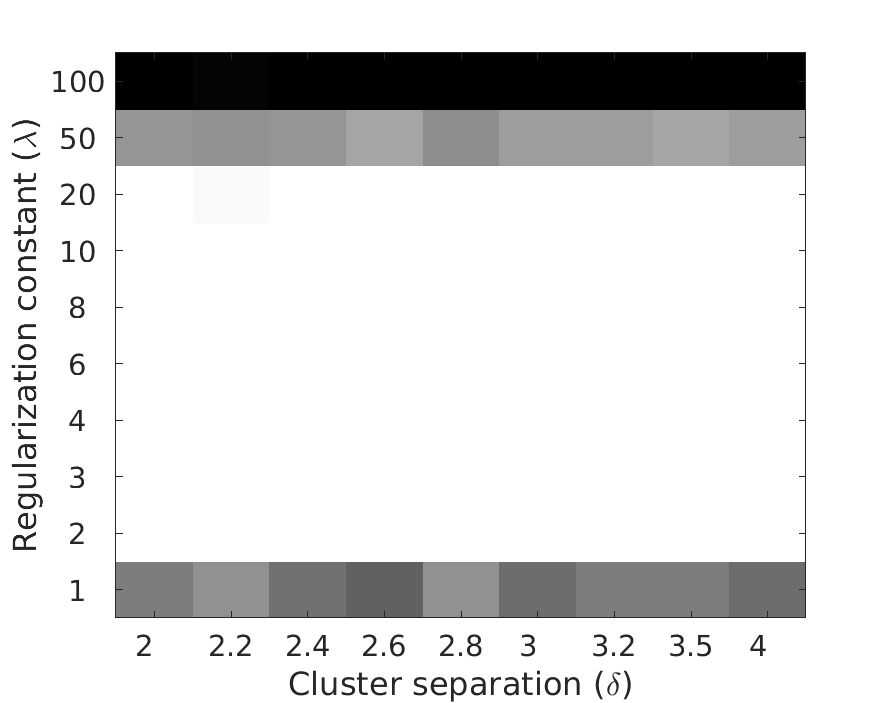
\includegraphics[width=0.45\textwidth]{figures/optimizationClustering/deltaLambda.png}
  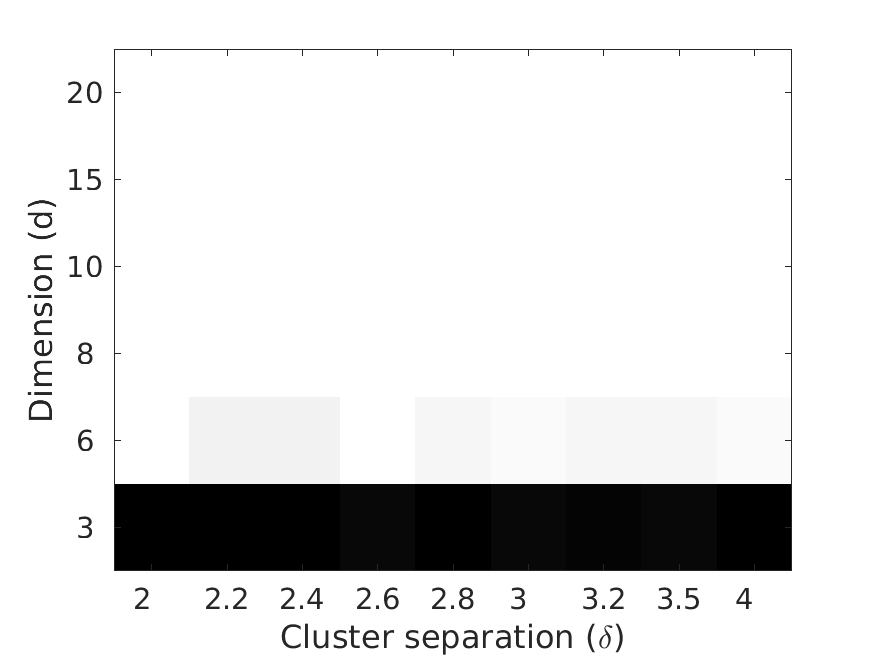
\includegraphics[width=0.45\textwidth]{figures/optimizationClustering/deltaD.png}
  \caption{Heatmap showing the probability of success of the $k$-means regularised sdp algorithm. Lighter color indicates probability closer to one while darker indicates probability closer to zero.}
\end{figure}
\begin{figure}
  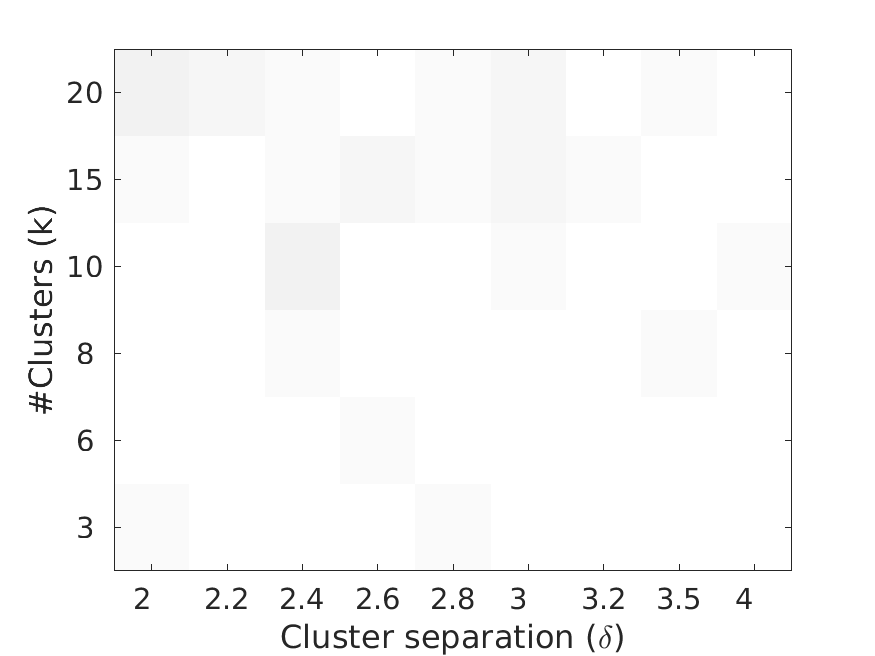
\includegraphics[width=0.45\textwidth]{figures/optimizationClustering/deltaK.png}
  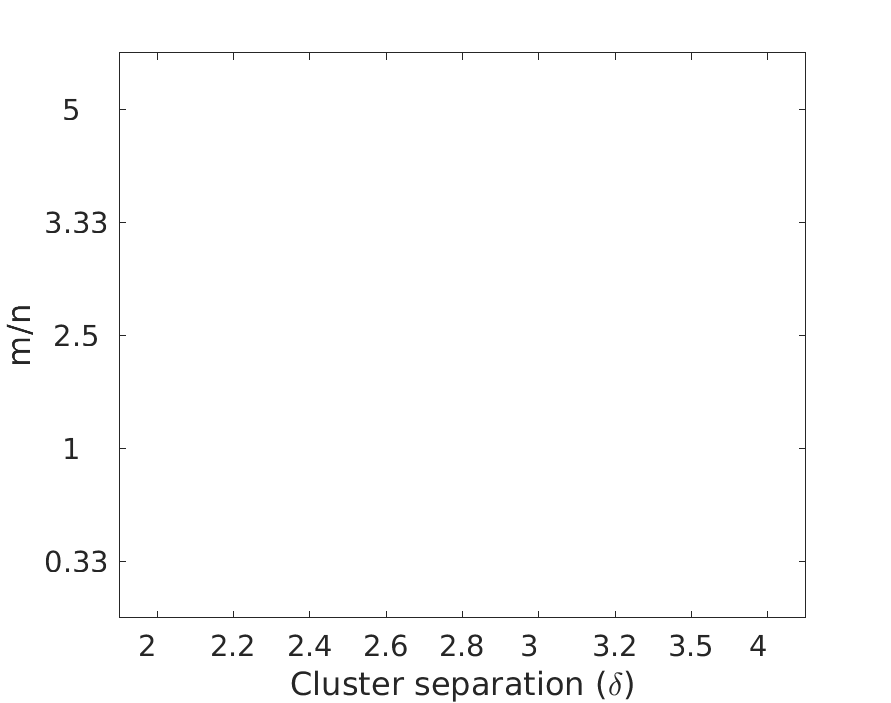
\includegraphics[width=0.45\textwidth]{figures/optimizationClustering/deltaM.png}
  \caption{Heatmap showing the probability of success of the $k$-means regularised sdp algorithm. Lighter color indicates probability closer to one while darker indicates probability closer to zero.$m$ denotes the number of noisy points while $n$ denotes the number of points in the smallest cluster.}
\end{figure}
\begin{figure}
  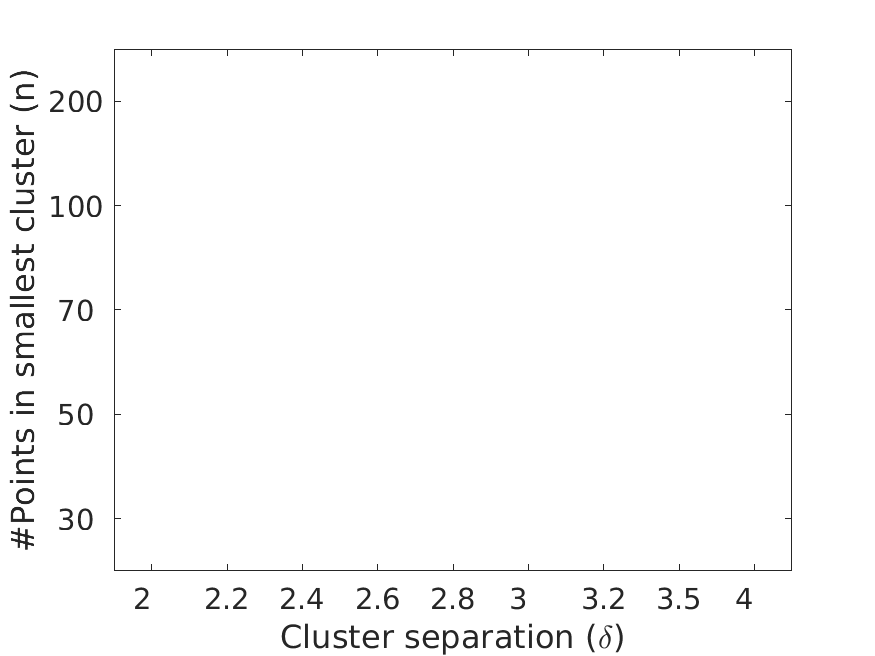
\includegraphics[width=0.45\textwidth]{figures/optimizationClustering/deltan.png}
  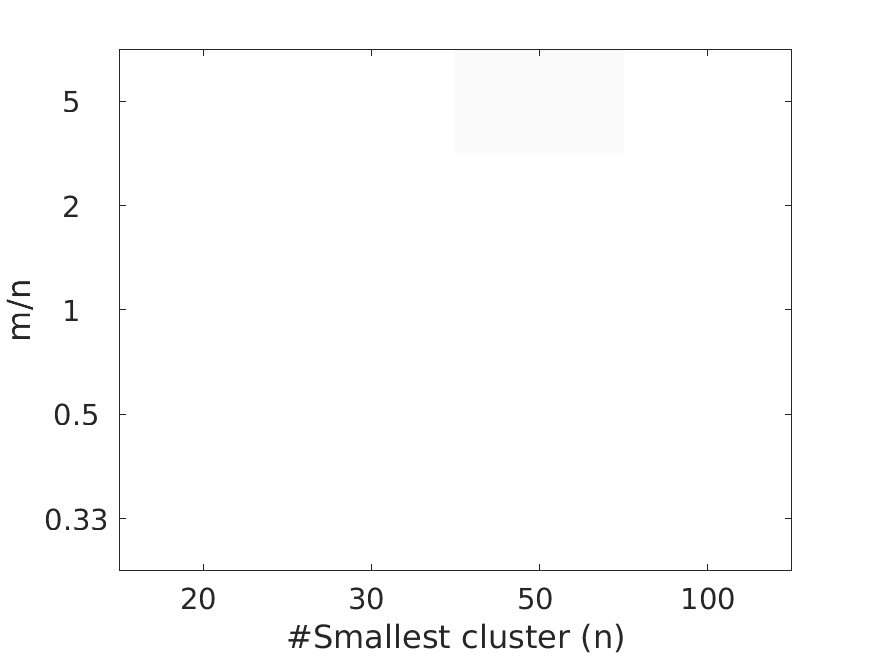
\includegraphics[width=0.45\textwidth]{figures/optimizationClustering/nM.png}
  \caption{Heatmap showing the probability of success of the $k$-means regularised sdp algorithm. Lighter color indicates probability closer to one while darker indicates probability closer to zero. $m$ denotes the number of noisy points while $n$ denotes the number of points in the smallest cluster.}  
\end{figure}

\section{Technical lemma}
\begin{theorem}[Thm. 5.41 in \cite{vershynin2010introduction}]
\label{a-thm:spectralNormCOncentration}
Let $A$ be an $N\times d$ matrix whose rows $A_i$ are independent isotropic random vectors in $\mb R^d$. Let $m$ be a number such that $\|A_i\| \le \sqrt{m}$ almost surely for all $i$. Then for every $t$, one has
$$\sqrt{N} - t\sqrt{m} \le \sigma_{\min}(A) \le \sigma_{\max}(A) \le \sqrt{N} + t\sqrt{m}$$
with probability atleast $1-2d\exp(-ct^2)$, where $c$ is an absolute constant. $\sigma_{\min}$ and $\sigma_{\max}$ are the spectral norms or the minimum and maximum eigenvalues respectively of the matrix $A$.
\end{theorem}

\ifdefined\COMPLETE
\else
\end{document}
\fi